\documentclass{misisarticle}

\usepackage{float}
\usepackage{flafter}
\usepackage[section]{placeins}

\grnti{28.23.15, 28.23.37}
\asjc{1702, 1707}
\oecd{1.02.EP}

\title{Сравнительный анализ нейросетевых моделей монокулярной оценки глубины в задаче определения траектории движения велосипеда по видео}

\misisauthor{А.~Р.~Прянишникова}{кафедра инженерной кибернетики НИТУ <<МИСиС>>}{Москва, Россия}{m2508848@edu.misis.ru}

\setabstract{В статье рассматривается проблема автоматического определения траектории движения велосипеда по видеозаписи~--- задача, имеющая значение для систем компьютерного зрения, навигации и анализа движения объектов. Данный подход позволяет восстановить путь перемещения по данным одной камеры без использования дополнительных сенсоров. Для решения поставленной задачи разработан метод, основанный на анализе последовательности видеокадров с применением алгоритмов оптического потока и нейросетевых моделей монокулярной оценки глубины. В результате исследования проведено сравнение трех открытых моделей оценки глубины Depth Anything V2 Metric Outdoor Small, Depth Anything V2 Metric Outdoor Base и ZoeDepth KITTI, а также выполнена оценка точности восстановления полученных траекторий.}

\setkeywords{визуальная одометрия, глубина сцены, компьютерное зрение, нейронные сети, оптический поток, траектория}

\begin{document}
\maketitle

\section{Введение}

В настоящее время методы компьютерного зрения являются практически незаменимыми в задачах анализа движения объектов и восстановления пространственной информации об окружающей среде. Одной из актуальных задач данного направления является определение траектории движения объекта по видеопоследовательности, полученной с помощью одной камеры. Такие методы позволяют создавать системы навигации и анализа движения без использования GPS-модулей или инерциальных датчиков. Современные методы, основанные на нейронных сетях, позволяют достигать высокой точности даже в сложных условиях~--- при разном уровне освещённости и на разной местности~\cite{ref1}.

Особый интерес представляет задача восстановления траектории движения велосипеда по видеозаписи. Данный подход может применяться для анализа маршрутов, построения карт окружающей среды, спортивной аналитики и разработки автономных систем навигации.

Одним из подходов к решению данной задачи является использование методов визуальной одометрии, основанных на анализе последовательности изображений для оценки перемещения камеры в пространстве. Для получения информации о трехмерной структуре сцены применяются методы монокулярной оценки глубины, позволяющие определять расстояние до объектов по одному изображению.

Методы глубокого обучения с использованием нейросетевых моделей оценки глубины позволяют автоматически выделять пространственные признаки из изображений и формировать карты глубины высокой детализации. Такие модели показали высокую эффективность в задачах компьютерного зрения, включая восстановление трехмерной структуры сцены и анализ изображений.

Depth Anything V2 является семейством нейросетевых моделей монокулярной оценки глубины, предназначенных для получения метрических карт глубины различных типов сцен. Модели данного семейства используют современные архитектуры глубокого обучения и позволяют получать точные оценки глубины при обработке изображений.

ZoeDepth также является нейросетевой моделью оценки глубины, ориентированной на получение метрических значений глубины и способной работать с различными типами сцен. Использование данной модели позволяет провести сравнение различных подходов к оценке глубины в задаче восстановления траектории движения.

Таким образом, сравнительный анализ нейросетевых моделей монокулярной оценки глубины в задаче определения траектории движения велосипеда по видео позволяет оценить влияние различных подходов к восстановлению пространственной информации и выбрать наиболее эффективные методы для дальнейшего применения в системах компьютерного зрения.

\section{Наборы данных}

В качестве наборов данных были записаны несколько велосипедных треков с камерой, закрепленной на руле велосипеда. Велосипедные треки записаны в разных условиях (например, в поселковой местности или в парке) и на различных маршрутах, включающих в себя повороты и прямые отрезки.

Также для получения эталонной траектории для каждого маршрута был записан трек в формате GPX (GPS eXchange Format).

GPX~--- это открытый формат хранения и обмена данными о маршрутах, основанный на языке разметки XML. Формат используется для представления информации о перемещении объектов и поддерживается большинством навигационных сервисов и устройств. Основным элементом GPX является набор точек пути, каждая из которых содержит географические координаты~--- широту и долготу, а также может включать дополнительные параметры, такие как высота, время записи и скорость движения.

\section{Нейросетевая архитектура}

\subsection{Методы монокулярной оценки глубины}

Монокулярная оценка глубины (сокращенно MDE)~--- это задача определения глубины по одному RGB-изображению~\cite{ref2}.

Изначально методы оценки глубины основывались преимущественно на геометрических подходах, таких как стереосопоставление и методы анализа движения камеры. Однако такие методы требуют наличия нескольких изображений, точной калибровки камер или дополнительных сенсоров. Развитие методов глубокого обучения позволило формулировать задачу оценки глубины как задачу прогнозирования плотной карты глубины непосредственно по изображению. Современные нейросетевые методы способны автоматически выделять пространственные признаки и получать более устойчивые оценки глубины для различных типов сцен.

В рамках методов монокулярной оценки глубины, основанных на self-supervised learning, часто используется архитектура, состоящая из двух основных компонентов: сети глубины и сети позы. Сеть глубины выполняет оценку карты глубины для входного изображения. Сеть позы используется для определения собственного движения камеры между последовательными кадрами видеопоследовательности. Совместное использование этих компонентов позволяет восстанавливать пространственную структуру сцены без необходимости наличия размеченных карт глубины~\cite{ref3}.

В отличие от self-supervised подходов, современные модели метрической оценки глубины, такие как Depth Anything V2 и ZoeDepth, обучаются на наборах данных с эталонными оценками глубины и позволяют напрямую получать карту глубины по одному изображению.

\subsubsection{Depth Anything V2}

Depth Anything V2 разрабатывалась как универсальная модель оценки глубины, способная работать с различными типами сцен и обладать высокой устойчивостью при обработке изображений, отличающихся от обучающих данных.

В основе обучения данной модели используется подход teacher--student, при котором сначала создается большая модель-учитель, обучаемая на синтетических данных и способная получать качественные оценки глубины. Затем ее предсказания используются для обучения меньших моделей. Таким образом, student-модели получают возможность использовать знания большой модели без необходимости обучения на больших объемах размеченных данных.

Depth Anything V2 включает в себя два основных компонента: DINOv2 Vision Transformer для извлечения признаков изображения и DPT (Dense Prediction Transformer) для преобразования признаков в карту глубины~\cite{ref4}. Такой состав обеспечивает высокую детализацию выходной карты глубины при сложных условиях съемки, включая низкую освещенность и помехи~\cite{ref5}.

DINOv2 Encoder анализирует изображение, выделяет семантические и пространственные признаки и затем формирует представление сцены.

DPT-декодер получает признаки от encoder и преобразует их в плотную карту глубины. На выходе модель формирует изображение, где каждому пикселю соответствует значение глубины.

Данная модель выпускается в нескольких типах, которые отличаются количеством параметров:
\begin{enumerate}[leftmargin=0.9cm,topsep=0pt,itemsep=0pt]
  \item Depth-Anything-V2-Small~--- 24{,}8 млн параметров;
  \item Depth-Anything-V2-Base~--- 97{,}5 млн параметров;
  \item Depth-Anything-V2-Large~--- 335{,}3 млн параметров.
\end{enumerate}

Чем больше параметров в модели, тем медленнее и требовательнее к ресурсам становится инференс.

\subsubsection{ZoeDepth KITTI}

ZoeDepth~--- это нейросетевая модель монокулярной оценки глубины, предназначенная для получения метрических карт глубины. Модель объединяет два подхода к построению карт глубины: relative depth estimation (оценка относительной глубины) и metric depth estimation (оценка абсолютной глубины в физических единицах)~\cite{ref6}.

Модель состоит из двух основных частей: основная сеть оценки относительной глубины MiDaS и специальный модуль, отвечающий за преобразование относительной глубины в метрическую.

Глубина определяется в несколько этапов:
\begin{enumerate}[leftmargin=0.9cm,topsep=0pt,itemsep=0pt]
  \item диапазон возможных глубин разделяется на несколько интервалов;
  \item определяется вероятность принадлежности пикселя к каждому интервалу;
  \item итоговая глубина вычисляется на основе полученного распределения.
\end{enumerate}

Версия модели ZoeDepth KITTI ориентирована на наружные сцены за счет обучения на изображениях с автомобильных камер, сценах городских дорог и данных о глубине от LiDAR~\cite{ref6}.

\section{Архитектура пайплайна определения траектории}

Для определения траектории движения велосипеда был разработан метод, основанный на совместном применении алгоритма оценки оптического потока и нейросетевых моделей монокулярной оценки глубины.

Общий алгоритм восстановления траектории состоит из шести этапов:
\begin{enumerate}[leftmargin=0.9cm,topsep=0pt,itemsep=0pt]
  \item из видео извлекаются отдельные кадры;
  \item производится оценка оптического потока с помощью модели RAFT Large~\cite{ref7};
  \item выполняется компенсация движений камеры, не обусловленных поворотом непосредственно велосипеда. Обработка видеопотока камер портативных устройств сопровождается рядом технических проблем, связанных с неконтролируемыми условиями съемки (освещение, ракурс, движение и пр.)~\cite{ref8}. После компенсации остается преимущественно компонент движения, связанный с реальным перемещением велосипеда;
  \item с помощью моделей монокулярной оценки глубины формируется карта метрической глубины. Полученные карты используются для преобразования двумерных координат точек изображения в трехмерные координаты пространства;
  \item производится оценка переноса камеры и сглаживание полученной траектории;
  \item для оценки качества восстановления полученные маршруты сравниваются с эталонной траекторией из GPX-файла.
\end{enumerate}

\section{Анализ результатов}

Рассмотрим работу пайплайна на маршруте, представленном на рисунке~\ref{fig:route1}.

\begin{figure}[!tbp]
  \centering
  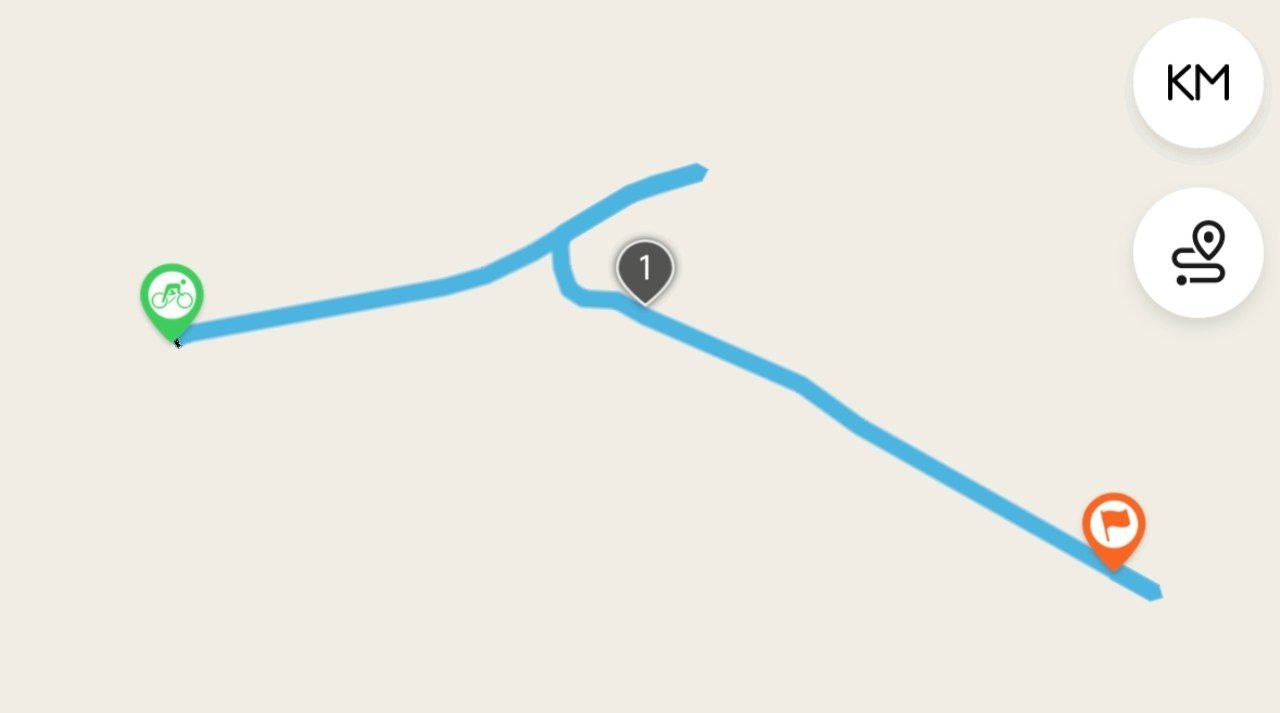
\includegraphics[width=\columnwidth]{figures/article/image2.jpeg}
  \caption{Вариант маршрута, на котором осуществлялась съемка}
  \label{fig:route1}
\end{figure}

Примеры кадров из маршрута представлены на рисунке~\ref{fig:frames1}. В результате работы пайплайна были получены траектории, представленные на рисунке~\ref{fig:trajectories1}.

\begin{figure}[!tbp]
  \centering
    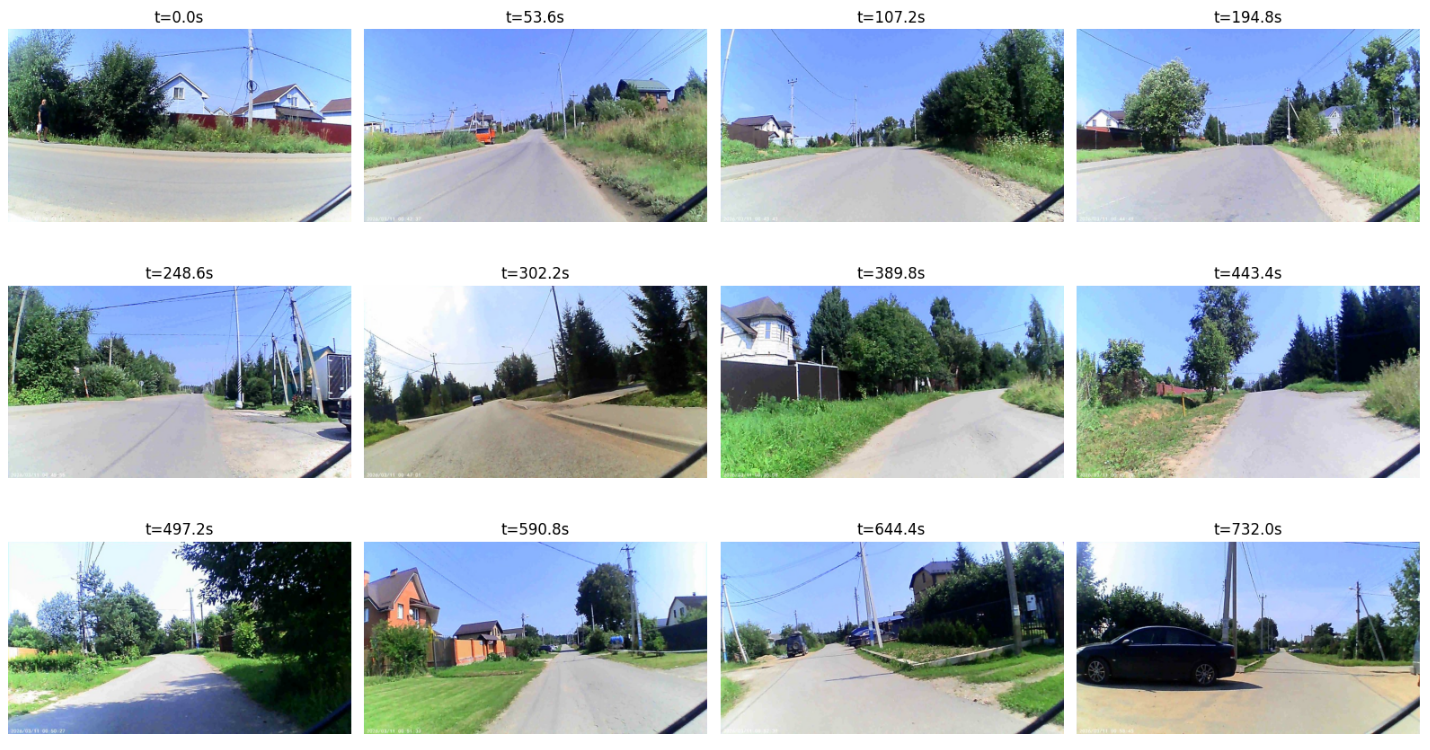
\includegraphics[height=4.2cm]{figures/article/image3.png}
    \caption{Примеры кадров из маршрута}
    \label{fig:frames1}
\end{figure}

\begin{figure}[!tbp]
  \centering
    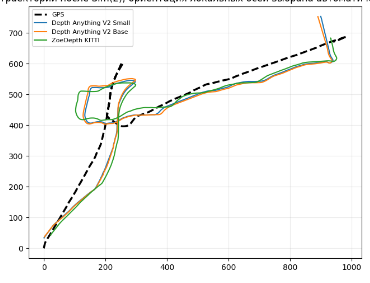
\includegraphics[height=4.2cm]{figures/article/trajectories1.png}
    \caption{Получившиеся траектории}
    \label{fig:trajectories1}
\end{figure}
\FloatBarrier

Для оценки работы пайплайна и влияния выбора модели монокулярной оценки глубины использовалась абсолютная ошибка траектории относительно эталонного GPS-маршрута. Ошибка измеряется в метрах; чем меньше ее значение, тем точнее восстановлена траектория.

На рисунке~\ref{fig:absolute1} приведен график абсолютной ошибки для каждой из трех моделей.

\begin{figure}[H]
  \centering
  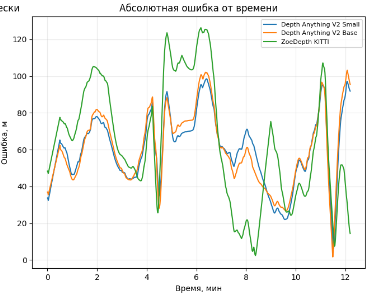
\includegraphics[width=0.74\columnwidth]{figures/article/trajectories2.png}
  \caption{График зависимости абсолютной ошибки от времени}
  \label{fig:absolute1}
\end{figure}

Результаты эксперимента показывают, что предложенный пайплайн позволяет восстановить пространственную траекторию движения велосипеда по видеопоследовательности для всех трех исследуемых моделей монокулярной оценки глубины. После выравнивания траекторий восстановленные маршруты сохраняют характерную форму движения и основные изменения направления, что подтверждает применимость монокулярной оценки глубины совместно с визуальной одометрией для решения поставленной задачи.

По абсолютной ошибке траектории Depth Anything V2 Metric Outdoor Base показывает лучший результат среди сравниваемых моделей.

\FloatBarrier

Рассмотрим работу пайплайна на маршруте более простой формы. Записываемая на камеру часть начинается с черного участка. Маршрут представлен на рисунке~\ref{fig:route2}.

\begin{figure}[H]
  \centering
  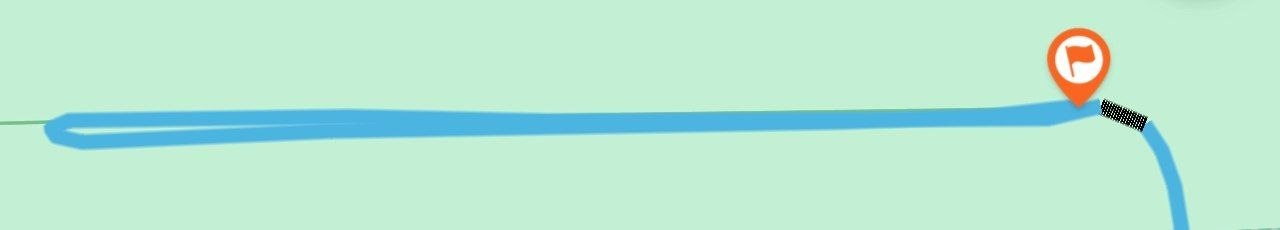
\includegraphics[width=\columnwidth]{figures/article/image10.png}
  \caption{Маршрут, на котором осуществлялась съемка}
  \label{fig:route2}
\end{figure}

Примеры кадров из маршрута представлены на рисунке~\ref{fig:frames2}.

\begin{figure}[H]
  \centering
  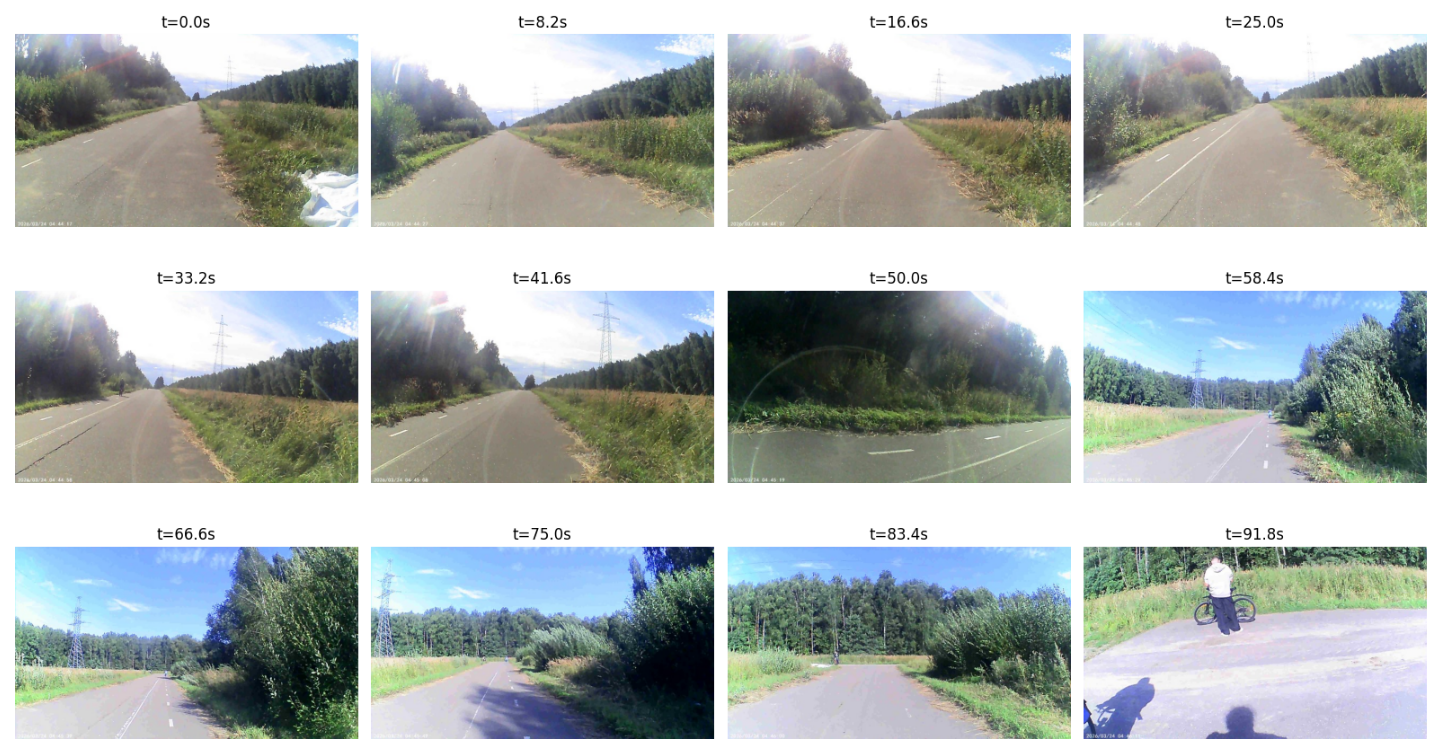
\includegraphics[width=\columnwidth]{figures/article/image11.png}
  \caption{Примеры кадров из маршрута}
  \label{fig:frames2}
\end{figure}

В результате работы пайплайна были получены траектории, представленные на рисунке~\ref{fig:trajectories2}.

\begin{figure}[H]
  \centering
  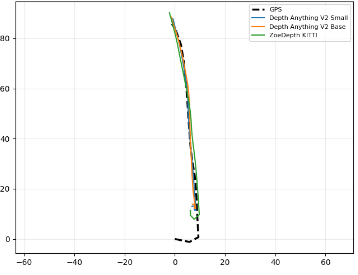
\includegraphics[width=0.82\columnwidth]{figures/article/absolute1.png}
  \caption{Получившиеся траектории}
  \label{fig:trajectories2}
\end{figure}

На рисунке~\ref{fig:absolute2} приведен график абсолютной ошибки для каждой из трех моделей.

\begin{figure}[H]
  \centering
  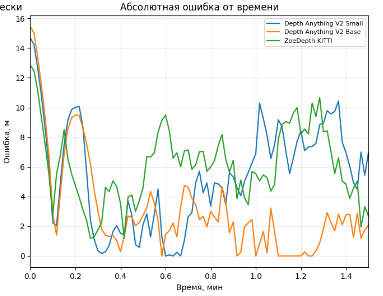
\includegraphics[width=0.82\columnwidth]{figures/article/absolute2.png}
  \caption{График зависимости абсолютной ошибки от времени}
  \label{fig:absolute2}
\end{figure}

\FloatBarrier

На данном исследуемом маршруте все три модели монокулярной оценки глубины обеспечили устойчивое восстановление траектории движения велосипеда. После пространственного выравнивания восстановленные траектории в значительной степени совпадают с эталонным GPS-маршрутом и корректно передают основное направление движения. При этом результаты различных моделей близки между собой, что свидетельствует об устойчивости предложенного пайплайна к выбору конкретной модели оценки глубины.

Значение абсолютной ошибки траектории для всех моделей составляет около 7~м.

\section{Заключение}

В результате исследования было показано, что применение нейросетевых моделей монокулярной оценки глубины позволяет восстанавливать траекторию движения велосипеда по видеозаписи и достаточно точно передавать общую форму маршрута и изменения направления движения. Для трех исследуемых моделей~--- Depth Anything V2 Metric Outdoor Small, Depth Anything V2 Metric Outdoor Base и ZoeDepth KITTI~--- были получены сопоставимые значения абсолютной ошибки, что подтверждает устойчивость разработанного подхода к выбору конкретной модели глубины. На первом маршруте наименьшую абсолютную ошибку показала Depth Anything V2 Metric Outdoor Base.

В качестве дальнейшего развития исследования можно предложить увеличение количества и разнообразия тестовых маршрутов, исследование других моделей монокулярной оценки глубины, а также совершенствование этапов оценки движения камеры и компенсации ее вращений. Дополнительно перспективным направлением является исследование способов уменьшения накопления ошибки при восстановлении длинных траекторий.

\begin{thebibliography}{9}

\bibitem{ref1} Омеров М.~А., Фомин И.~Д. Исследование возможности детектирования и классификации видов транспорта с помощью современных технологий машинного зрения~// Искусственный интеллект в промышленных, коммерческих, медицинских и финансовых приложениях: сб. статей научно-технического семинара студентов кафедры «Инженерной кибернетики», Москва, 30 мая 2025 года. М.: НИТУ «МИСИС», 2025. С.~89--94. EDN ABCXIR.

\bibitem{ref2} Bhoi A. Monocular Depth Estimation: A Survey~// arXiv. 2019. No.~1901.09402. URL: https://arxiv.org/abs/1901.09402 (дата обращения: 29.08.2026).

\bibitem{ref3} Masoumian A., Rashwan H.~A., Cristiano J., Asif M.~S., Puig D. Monocular Depth Estimation Using Deep Learning: A Review~// Sensors (Basel). 2022. Vol.~22, no.~14. Art.~5353. DOI: https://doi.org/10.3390/s22145353. PMID: 35891033; PMCID: PMC9325018.

\bibitem{ref4} Yang L., Kang B., Huang Z., Zhao Z., Xu X., Feng J., Zhao H. Depth Anything V2~// arXiv. 2024. No.~2406.09414. URL: https://arxiv.org/abs/2406.09414 (дата обращения: 29.08.2026).

\bibitem{ref5} Быкова А.~О., Рублева С.~С. Детектирование опасного вождения на основе фиксации вибрации камеры с применением нейросетевых архитектур MiDaS и Depth Anything V2~// Искусственный интеллект в промышленных, коммерческих, медицинских и финансовых приложениях: сб. статей научно-технического семинара кафедры «Инженерной кибернетики», Москва, 26 июня 2026 года. Вып.~6. М.: НИТУ «МИСИС», 2026. С.~4--10.

\bibitem{ref6} Bhat S.~F., Birkl R., Wofk D., Wonka P., Müller M. ZoeDepth: Zero-shot Transfer by Combining Relative and Metric Depth~// arXiv. 2023. No.~2302.12288. URL: https://arxiv.org/abs/2302.12288 (дата обращения: 29.08.2026).

\bibitem{ref7} Teed Z., Deng J. RAFT: Recurrent All-Pairs Field Transforms for Optical Flow~// arXiv. 2020. No.~2003.12039. URL: https://arxiv.org/abs/2003.12039 (дата обращения: 29.08.2026).

\bibitem{ref8} Солодов С.~В., Проничкин С.~В. Методы исследования дефектов дорожного покрытия в видеопотоке камер портативных устройств~// Новые материалы и перспективные технологии: сб. материалов Пятого междисциплинарного научного форума с международным участием, Москва, 30 октября~-- 1 ноября 2019 года. Т.~I. М.: Интеллектуальные системы, 2019. С.~418--421. EDN SZLIDC.

\end{thebibliography}

\end{document}
